%----------------------------------------------------------------------------------------
%	PACKAGES AND OTHER DOCUMENT CONFIGURATIONS
%----------------------------------------------------------------------------------------

\documentclass{article} % Paper and 12pt font size
\usepackage[utf8]{inputenc}
\usepackage{lmodern} % Use font Latin Modern Sans Typewriter
\usepackage[a4paper, margin=1in]{geometry} % Paper size and margin

\usepackage{enumitem} % Format the enumerated list
\usepackage{amsmath,amsfonts,amsthm,mathtools} % Math packages
\setlength\parindent{0pt} % Removes all indentation from paragraphs - comment this line for an assignment with lots of text

\usepackage{array}
\usepackage{tabu} % Table to text width
\renewcommand{\arraystretch}{0.6} % If the value is 1.0, the height of each row in the table is set to 1.5 relative to its default height. Adjust based on that.
\usepackage[table]{xcolor}

\usepackage{tikz} % Remember picture
\usepackage{graphicx} % Includes images
\graphicspath{ {./images/} } % Tells LATEX that the images are kept in a folder named images under the directory of the main document
\usepackage{subcaption}
\usepackage{wrapfig} % Wrap image i
\usepackage{eso-pic} % used for image background on titlepage

% Code listing style --------------
\usepackage{listings} % Code listing
\usepackage{color}
\definecolor{codegreen}{rgb}{0,0.6,0}
\definecolor{codegray}{rgb}{0.5,0.5,0.5}
\definecolor{codepurple}{rgb}{0.58,0,0.82}
\definecolor{backcolour}{rgb}{0.95,0.95,0.92}
\lstdefinestyle{mystyle}{
    backgroundcolor=\color{backcolour},
    commentstyle=\color{codegreen},
    basicstyle=\ttfamily\small,
    keywordstyle=\color{magenta},
    numberstyle=\tiny\color{codegray},
    stringstyle=\color{codepurple},
    breakatwhitespace=false,
    breaklines=true,
    captionpos=b,
    keepspaces=true,
    numbers=left,
    numbersep=5pt,
    showspaces=false,
    showstringspaces=false,
    showtabs=false,
    tabsize=2
}
\lstset{style=mystyle}

%----------------------------------------------------------------------------------------
%	TITLE SECTION
%----------------------------------------------------------------------------------------
\title{\Huge \textbf{Report on K-NN Algorithm in Classification and Regression} \vspace{.4in} \hrule}

\author{%\LARGE University of Toronto Institute for Aerospace Studies\\
  \vspace{0.5cm}
	\Large ROB313: Introduction to Learning from Data \\
  \vspace{0.5cm}
	\Large Yizhi (Jojo) Zhou, 1003002396\\
}
\date{\normalsize\today}

\linespread{1.5}

\begin{document}
	\begin{titlepage}
	\tikz[remember picture,overlay]
	\node[yshift=8.0cm] at (current page.south){
\includegraphics[width=\paperwidth]{404.png}};%height=\paperheight and (current page.south)
	\vspace*{3.5cm}
  {\let\newpage\relax\maketitle}
	\vspace*{\fill}

	\end{titlepage}

\newpage

%----------------------------------------------------------------------------------------
%	PROBLEM 1
%----------------------------------------------------------------------------------------
\vspace{0.4cm}
\section*{Objectives} % The * makes it an unnumbered section
The k-nearest neighbors algorithm (k-NN) is an pattern recognition method used for classification and regression, where the prediction is approximated from the k closest training examples in the feature space. This project cross-validates and tests k-NN with different distance metrics and k-values on five sets of regression and training data, aiming to find the optimal distance metric and k for each dataset and study the relationship between each input parameter and output prediction.

Then, different data structures, ranging from brutal force to vectorization and kd-trees, are compared in terms of their run-times, for comparing the performance of each data structures in k-NN with different feature space dimensions. Finally, k-NN is compared to linear regression and the results will be discussed in the following report.


%----------------------------------------------------------------------------------------
%	PROBLEM 1
%----------------------------------------------------------------------------------------
\vspace{0.4cm}
\section*{Solution Structure and Strategies} % The * makes it an unnumbered section
The first half of solution, the implementation of k-NN, is composed of three main sections: data processing, training, and validation/testing. They are separated in three different input cells in the Jupyter Notebook\footnote{The Jupyter Notebook is attached in the submitted folder.} Details are indicated below:
\begin{itemize}
  \item \textbf{Preprocessing.} This section  simply loads the specified dataset and concatenates the training and validation sets. It then normalizes all the features with respect to the mean and standard deviation of this concatenated training-validation set.
  For future cross-validation, all the indices of the concatenated set is randomized and passed on to a folding function that splits it into two portions with length ratio 4:1. The elements corresponding to these two sets of indices becomes the training and validation set.
  \item \textbf{Training.} Object-oriented programming is used here for easier repeated extraction of data. The training class contains 4 functions that outputs the prediction:
    \begin{itemize}
    \item \textit{kNNRegression} extracts the k nearest neighbours of the input feature data with the helper functions below, computes the average of their corresponding label values, and outputs this average as the prediction along with its error compared to the actual value.
      \begin{itemize}
      \item \textit{getDistance} computes the specified distance (eg. $l_2$) between two input vectors.
      \item \textit{getNeighbours} passes each vector in the training set into the \textit{getDistance} function with the feature vector to be predicted. It then finds the k smallest numbers from all the distances and returns a list of indices corresponding to these distances. \textit{getNeighbours\_2} produces the same result, while replacing the iteration with \textit{numpy}'s broadcasting.
    \end{itemize}
    \item \textit{kNNRegression\_3} serves the same functionality as  \textit{kNNRegression}, while using vectorization to fully replace the iterations. This is done by duplicating the training set into another dimension that has the same size as the set to be predicted.
    \item \textit{kNNRegression\_4} also serves the same functionality, while turning the training set into a kd tree structure to find the nearest neighbours' indices for the set to be predicted.
    \item \textit{kNNClassification} follows the same algorithm as \textit{kNNRegression}, extracting the k-nearest neighbours. The prediction is thus the class with the most votes in these k neighbours.
  \end{itemize}
  \item \textbf{Validation/Testing.} Multiple functions are implemented for the purpose of tuning, validation, and visualization. The \textit{RMSEComparison} function, for example, outputs the average root-mean-square error over the 5 cross-validation folds, for each dataset, each k, and each distance metric. There are also functions for plotting the prediction curve, visualizing the prediction, and comparing different algorithms' performance, etc. The results will be discussed in the following sections, and more details can be found in the Jupyter Notebook.
\end{itemize}
The second half of solution is linear regression:
\begin{itemize}
  \item \textbf{Linear Regression.} Also implemented in object-oriented programming, the linear regression is very similar to the training class of k-NN discussed above, except that an extra column of 1's is added to each feature vector before they are passed down.
  \begin{itemize}
    \item \textit{optimalWeight} computes the weight vector $w = V\Sigma^{-1}U^Ty$ with the economic SVD of the training set.
    \item \textit{linRegRegression} predicts $y = Xw$ and the corresponding root-mean-square error.
    \item \textit{linRegClassification} also computes $y = Xw$, but instead of being a scalar like in regression, $y$ is a vector whose each element is the likelihood of each class, and the prediction is therefore the class with the maximum likelihood.
  \end{itemize}
\end{itemize}



%----------------------------------------------------------------------------------------
%	PROBLEM 1
%----------------------------------------------------------------------------------------
\vspace{0.4cm}
\section*{k-NN on Regression} % The * makes it an unnumbered section

\textbf{Optimal k value \& distance metric}

  For each regression dataset, the k-NN algorithm is implemented with $l_2, l_1,$ and $l_{\inf}$ distances metrics and 15 different k values. The results are shown in the two tables below. The last row of each table indicates the average result over all tested k values with each distance metric, where the blue label indicates the optimal metric and the yellow label indicates the best performing k with this optimal distance metric.

  % Table for cross-validation
  \begin{table}[!ht]
  \begin{minipage}{0.33333\textwidth}
  \centering
  \scalebox{0.74}{\begin{tabular}[t]{||r | c c c||}
      \hline
      \rowcolor{lightgray}\multicolumn{4}{||c||}{ Dataset "mauna\_loa"}\\
      k  &\cellcolor{cyan}l1 & \cellcolor{cyan}l2 & \cellcolor{cyan}linf \\
      \hline
      1   & 0.048766  & 0.048766  & 0.048766 \\
      \cellcolor{yellow}2   &\cellcolor{yellow} 0.034748  &\cellcolor{yellow} 0.034748  &\cellcolor{yellow} 0.034748 \\
      3   & 0.042465  & 0.042465  & 0.042465 \\
      4   & 0.047779  & 0.047779  & 0.047779 \\
      5   & 0.056833  & 0.056833  & 0.056833 \\
      6   & 0.064124  & 0.064124  & 0.064124 \\
      7   & 0.072076  & 0.072076  & 0.072076 \\
      8   & 0.078499  & 0.078499  & 0.078499 \\
      9   & 0.084152  & 0.084152  & 0.084152 \\
      10  & 0.088429  & 0.088429  & 0.088429 \\
      11  & 0.091492  & 0.091492  & 0.091492 \\
      12  & 0.093084  & 0.093084  & 0.093084 \\
      13  & 0.093264  & 0.093264  & 0.093264 \\
      14  & 0.092027  & 0.092027  & 0.092027 \\
      15  & 0.090025  & 0.090025  & 0.090025 \\
      \hline
      Avg&\cellcolor{cyan}  0.069534 &\cellcolor{cyan} 0.069534 &\cellcolor{cyan}  0.069534 \\
      \hline
      \rowcolor{pink}\multicolumn{4}{||c||}{Test Set RMSE: 0.249432}\\
      \hline
  \end{tabular}}
  \end{minipage}
  \begin{minipage}{0.33333\textwidth}
  \centering
  \scalebox{0.74}{\begin{tabular}[t]{||r | c c c||}
      \hline
      \rowcolor{lightgray}\multicolumn{4}{||c||}{ Dataset "rosenbrock"}\\
      k  &       l1 & \cellcolor{cyan}l2 &      linf \\
      \hline
      \cellcolor{yellow}1   & 0.332775  & \cellcolor{yellow}0.302071  & 0.284103 \\
      2   & 0.324385  & 0.313196  & 0.306085 \\
      3   & 0.326387  & 0.314938  & 0.316781 \\
      4   & 0.340917  & 0.340087  & 0.324859 \\
      5   & 0.358044  & 0.341096  & 0.346290 \\
      6   & 0.364532  & 0.350955  & 0.359211 \\
      7   & 0.384731  & 0.363403  & 0.371243 \\
      8   & 0.387628  & 0.374365  & 0.381987 \\
      9   & 0.388331  & 0.382530  & 0.399302 \\
      10  & 0.395729  & 0.393533  & 0.405465 \\
      11  & 0.411511  & 0.404733  & 0.415856 \\
      12  & 0.422927  & 0.417982  & 0.422297 \\
      13  & 0.431890  & 0.431304  & 0.430378 \\
      14  & 0.440227  & 0.437629  & 0.445694 \\
      15  & 0.446847  & 0.448048  & 0.453156 \\
      \hline
      Avg&  0.383791 & \cellcolor{cyan}0.374391 &  0.377514 \\
      \hline
      \rowcolor{pink}\multicolumn{4}{||c||}{Test Set RMSE: 0.237871}\\
      \hline    \end{tabular}}
  \end{minipage}
  \begin{minipage}{0.33333\textwidth}
  \centering
  \scalebox{0.74}{\begin{tabular}[t]{||r | c c c||}
      \hline
      \rowcolor{lightgray}\multicolumn{4}{||c||}{ Dataset "pumadyn32nm"}\\
      k  & \cellcolor{cyan}l1 &        l2 &      linf \\
      \hline
      25  & 0.872985  & 0.894633  & 0.970556 \\
      \cellcolor{yellow} 26  & \cellcolor{yellow} 0.872973  & 0.894929  & 0.970842 \\
      27  & 0.873117  & 0.895326  & 0.970808 \\
      28  & 0.873294  & 0.895341  & 0.970788 \\
      29  & 0.874463  & 0.895456  & 0.970688 \\
      30  & 0.874884  & 0.896378  & 0.970625 \\
      31  & 0.875496  & 0.896785  & 0.970095 \\
      32  & 0.875848  & 0.896747  & 0.969583 \\
      33  & 0.875969  & 0.897263  & 0.969211 \\
      34  & 0.875786  & 0.897464  & 0.968942 \\
      35  & 0.875514  & 0.897795  & 0.969062 \\
      36  & 0.876018  & 0.897742  & 0.969312 \\
      37  & 0.876163  & 0.897870  & 0.968781 \\
      38  & 0.875949  & 0.898411  & 0.968615 \\
      39  & 0.876167  & 0.898847  & 0.968634 \\
      \hline
      Avg& \cellcolor{cyan} 0.874975 &  0.896732 &  0.969769 \\
      \hline
      \rowcolor{pink}\multicolumn{4}{||c||}{Test Set RMSE: 0.831297}\\
      \hline
  \end{tabular}} % end shrinksize
  \end{minipage}
  \caption{RMSE results of the cross-validation and test set of each regression dataset}
  \end{table}



  \begin{itemize}
    \item \textbf{mauna\_loa:} The optimal parameters are \textbf{k: $2$, any distance metrics}, where the test set produces an RMSE of 0.249432. It is worth noting that the distance metrics doesn't make a difference in finding neighbours in this dataset. This is because, since the features have only one dimension, the distance between two scalars has only one option, $|a-b|$. It is also noticable that the test set's RMSE is way larger than the validation sets', which will be discussed in the next part.
    \item \textbf{iris:} The optimal parameters are \textbf{k: $1$, distance metrics: $l_2$}, where the test set produces an RMSE of 0.237871, smaller than any of the validation sets'.
    \item \textbf{rosenbrock($n=1000$, $d=2$):} The optimal parameters are \textbf{k: $26$, distance metrics: $l_1$}, where the test set produces an RMSE of 0.831297. Note that the RMSE results with different k values are very similar in the range shown in the table and more data can be found in the Jupyter Notebook.
  \end{itemize}

\vspace{0.2cm}

\textbf{Prediction Performance on Dataset "mauna\_loa"}

  The validation and testinhg results are shown in Figure 1 and 2. It is obvious that the choice of optimal k, as well as the RMSE performance curve's general trend, varies significantly between the validation sets and test set. For example, the optimal k value shown by the cross-validation is 2 while that of the test set is 8. Meanwhile, it is shown in the previous part that the test set's RMSE is about 7 times larger than that of the validation sets.

    \begin{figure}[!b]
      \centering
      \begin{subfigure}[b]{0.45\linewidth}
        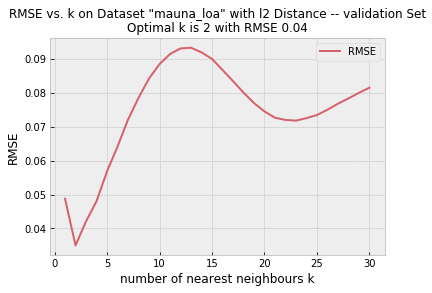
\includegraphics[width=\linewidth]{output_12_0.png}
        \caption{Cross validation}
      \end{subfigure}
      \begin{subfigure}[b]{0.45\linewidth}
        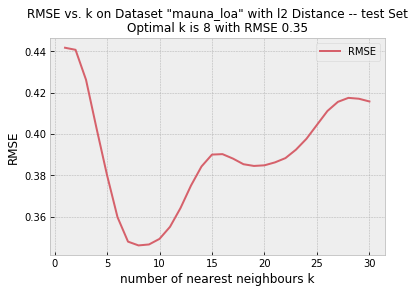
\includegraphics[width=\linewidth]{output_12_2.png}
        \caption{Test set}
      \end{subfigure}
      \caption{RMSE results with different k-values}
      \label{fig:Q1_1}
    \end{figure}

    \begin{figure}[!t]
      \centering
      \begin{subfigure}[b]{0.45\linewidth}
        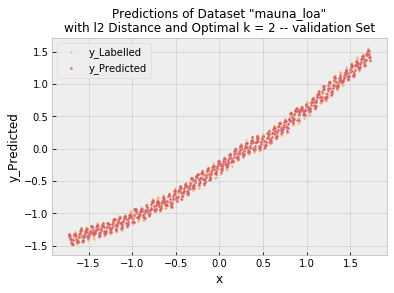
\includegraphics[width=\linewidth]{output_13_1.png}
        \caption{Cross validation}
      \end{subfigure}
      \begin{subfigure}[b]{0.45\linewidth}
        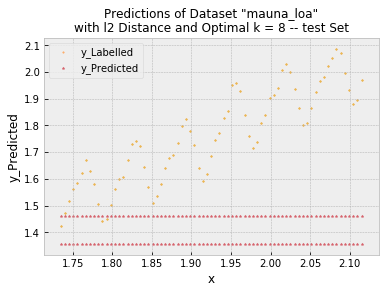
\includegraphics[width=\linewidth]{output_13_3.png}
        \caption{Test set}
      \end{subfigure}
      \caption{Prediction visualization at the optimal k}
      \label{fig:Q1_2}
    \end{figure}

  The reason behind this undesired performance is the distribution of data set. As a non-parametric technique, k-NN doesn't make any assumption on the underlying data distribution, which means that it is suitable for randomly distributed data, but can perform poorly if \textbf{the test points don't distribute randomly amoung the training points}. Since the features of mauna\_loa are actually years, there is a very clear and strong underlying trend which can't be captured by k-NN. Instead, because all the testing featrues are years after the training set, the closest neighbours are always the k largest x's in the training set (i.e. k latest years). Therefore, as indicated in Figure 2, where the predictions have the same value (about $1.34$ with $k=2$ and $1.46$ with $k=8$) because whether the normalized x is 1.75 or 2.10, the prediction is always the average of the k data points lying on the upper boundary of the training set.

  One way to make k-NN suitable on "mauna\_loa" is to recognize and counteract the underlying shape (i.e. linear/quadratic curve) of it by mapping the data points to a relatively uniform distribution. That being said, the brutal force implementation of k-NN is still a bad practice on a trended dataset like "mauna\_loa", where linear regression could perform much better as will be shown in the last section.



%----------------------------------------------------------------------------------------
%	PROBLEM 1
%----------------------------------------------------------------------------------------
\vspace{0.4cm}
\section*{k-NN on Classification} % The * makes it an unnumbered section

\textbf{Optimal k value \& distance metric}

  For each classification dataset, the k-NN algorithm is also implemented with $l_2, l_1,$ and $l_{\inf}$ distances metrics and 15 different k values. The results and optimal choices are shown in the two tables below.

  \begin{table}[!ht]
  \begin{minipage}{0.51\textwidth}
  \raggedleft
  \scalebox{0.74}{\begin{tabular}[t]{||r | c c c||}
    \hline
    \rowcolor{lightgray}\multicolumn{4}{||c||}{ Dataset "iris"}\\
    k  &       l1 &  \cellcolor{cyan} l2 &      linf \\
    \hline
    1   & 0.925926  & 0.925926  & 0.925926 \\
    2   & 0.940741  & 0.918519  & 0.911111 \\
    3   & 0.940741  & 0.948148  & 0.925926 \\
    4   & 0.948148  & 0.940741  & 0.911111 \\
    5   & 0.948148  & 0.955556  & 0.918519 \\
    6   & 0.940741  & 0.955556  & 0.911111 \\
    7   & 0.940741  & 0.962963  & 0.933333 \\
    8   & 0.940741  & 0.948148  & 0.940741 \\
    9   & 0.940741  & 0.962963  & 0.955556 \\
    10  & 0.948148  & 0.962963  & 0.948148 \\
    11  & 0.948148  & 0.962963  & 0.940741 \\
    \cellcolor{yellow}12  & 0.955556  & \cellcolor{yellow}0.962963  & 0.940741 \\
    13  & 0.948148  & 0.962963  & 0.933333 \\
    14  & 0.955556  & 0.955556  & 0.933333 \\
    15  & 0.948148  & 0.962963  & 0.933333 \\
    \hline
    Avg & 0.944691  & \cellcolor{cyan} 0.952593  & 0.930864 \\
    \hline
    \rowcolor{pink}\multicolumn{4}{||c||}{Test Set Accuracy: 1.0}\\
    \hline
  \end{tabular}}\hspace{0.02\textwidth}
  \end{minipage}
  \hspace{0.03\textwidth}\begin{minipage}{0.51\textwidth}
  \raggedright
  \scalebox{0.74}{\begin{tabular}[t]{||r | c c c||}
    \hline
    \rowcolor{lightgray}\multicolumn{4}{||c||}{ Dataset "mnist\_small"}\\
    k  & \cellcolor{cyan} l1 &        l2 &      linf \\
    \hline
    1  & 0.925000  & 0.908727  & 0.678545 \\
    2  & 0.918273  & 0.895364  & 0.648909 \\
    3\cellcolor{yellow} &\cellcolor{yellow} 0.929091  & 0.911636  & 0.670182 \\
    4  & 0.925636  & 0.908636  & 0.671727 \\
    5  & 0.927818  & 0.911636  & 0.669727 \\
    6   & 0.925545  & 0.908273  & 0.665364 \\
    7   & 0.925909  & 0.910273  & 0.664000 \\
    8   & 0.924182  & 0.906909  & 0.659364 \\
    9   & 0.923273  & 0.906364  & 0.660182 \\
    10  & 0.919455  & 0.904273  & 0.657455 \\
    11  & 0.918273  & 0.904000  & 0.658364 \\
    12  & 0.916000  & 0.901818  & 0.653273 \\
    13  & 0.916818  & 0.902455  & 0.651364 \\
    14  & 0.913091  & 0.901273  & 0.649364 \\
    15  & 0.913455  & 0.899636  & 0.649273 \\
    \hline
    Avg &\cellcolor{cyan} 0.921455  & 0.908727  & 0.660473 \\
    \hline
    \rowcolor{pink}\multicolumn{4}{||c||}{Test Set Accuracy: 0.937}\\
    \hline
  \end{tabular}}
  \end{minipage}
  \caption{Percentage accuracy (out of 1.0) of the cross-validation and test set of each classification dataset}
  \end{table}

  \begin{itemize}
    \item \textbf{iris:} The optimal parameters are \textbf{k: $12$, distance metrics: $l_2$}, where the test set is predicted $100\%$ correctly. Since the accuracies is generally similar amoung different k values, such as the highest $96.3\%$ which has occured multiple times, the optimal k value is determined by referencing the performance of $l_1$ and $l_{inf}$ as well. However, this also means that the optimal k value would easily be altered depending on the randomization of cross-validation. In fact, different k values around 12 have been tried and they all predicted perfectly.
    \item \textbf{mnist\_small:} The optimal parameters are \textbf{k: $12$, distance metrics: $l_1$}, where the test set is predicted correctly $93.7\%$ of the times. $l_1$ and $l_2$ gives a similar high accuracy of above $90\%$, but $l_{inf}$ performs significantly worse.
  \end{itemize}



%----------------------------------------------------------------------------------------
%	PROBLEM 1
%----------------------------------------------------------------------------------------
\vspace{0.4cm}
\section*{Runtime Performance with Different Implementations of k-NN} % The * makes it an unnumbered section
\begin{wrapfigure}{r}{0.49\textwidth}
  \centering
  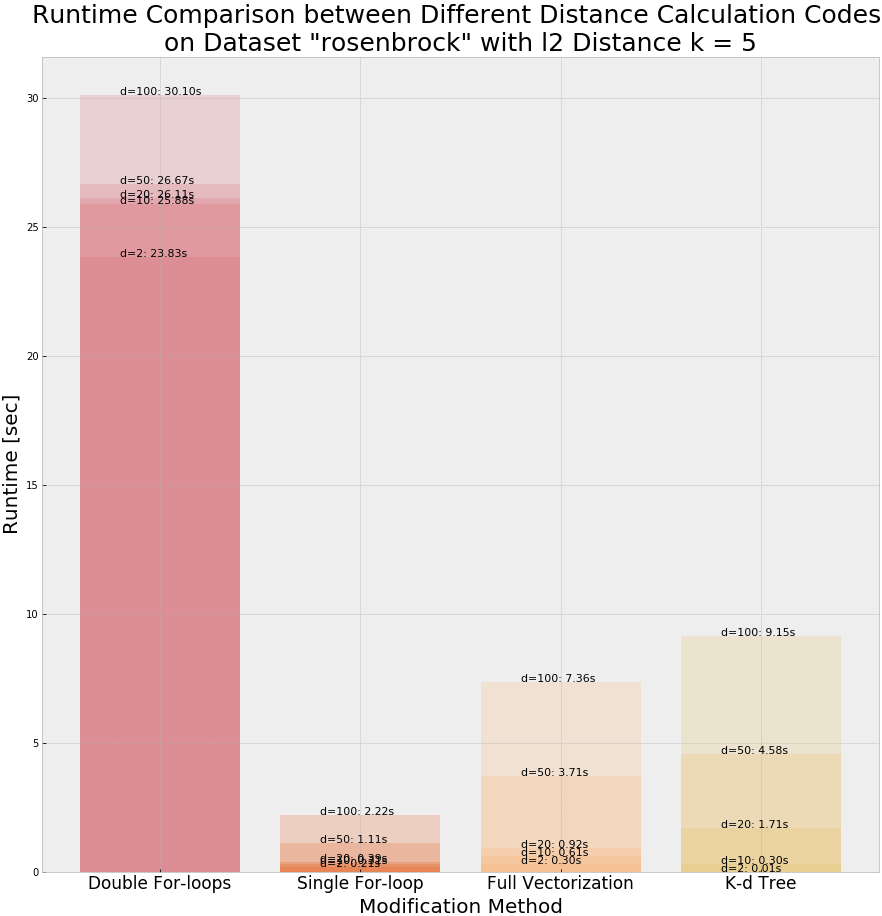
\includegraphics[width=0.49\textwidth]{kNNPerformance-TestSet-rosenbrock.png}
  \caption{Runtime performance of different implementations of k-NN}
\end{wrapfigure}

To test the difference in runtime performance of different k-NN implementations, 4 different structures are experimented with "rosenbrock" with 5000 training points, $k=5$, $l_2$ distance, and different feature dimentions ranging from 2 to 100.

\begin{itemize}
  \item The left most one of the highest runtime is the brutal force approach, where each testing point is looped through, comparing to each training point.

  \item The single for-loop implementation replaces latter loop by computing the distance between a broadcasted test point and all training points. It is found to be one order of magnitude faster than the brutal force, as the loop that costs $O(n)$ for each testing point is replaced at a small cost of vectorizing a test point with $n$ copies.
\end{itemize}

\begin{itemize}
  \item The remaining for-loop is now also replaced with full-vectorization where the training set is broadcasted to match the number of testing data so that the computation can be done directly between the two sets. It is, however, slower than the half-vectorization. This result could be because copying the $n$-by-$d$ tranining set multiple times requires allocating and filling such massive blocks of memory that it costs even more time than looping through the test set.

  \item Another way of replacing full loops is using a k-d tree data structure to compute the nearest neighbours for all test points simultaneously. This approach still performs a lot better than the brutal force one because of the faster searching on a k-d tree compared to that on a list. However, k-d tree's implementation in \textit{scikit-learn} uses the median rule, which is relatively expensive to build and worse for higher dimensions. Therefore, k-d tree's performance is the best amoung all implementations on low dimension data (i.e. $d=2$, $10$), but not as good when dimension increasies (i.e. $d>20$).
\end{itemize}



%----------------------------------------------------------------------------------------
%	PROBLEM 1
%----------------------------------------------------------------------------------------
\vspace{0.4cm}
\section*{Linear Regression vs. k-NN} % The * makes it an unnumbered section
A linear regressin algorithm that minimizes the least-squares loss is implemented with economic SVD. The accuracy performance of linear regression compared to k-NN on each dataset is listed in the table on the left. Linear regression predicts better only on "mauna\_loa", which has a nearly linear underlying shape, but doesn't perform as well as k-NN on any other dataset. The table on the right lists the runtine performance on "rosenbrock" with 5000 training points. The RMSE performance stays higher than that of k-NN, but the runtime is always nearly zero regardless of the dimension, showing that linear regression has a much more desireable computational cost on large datasets and/or large dimensions.
\begin{table}[!ht]
\begin{minipage}{0.44\textwidth}
\raggedleft
\scalebox{0.74}{\begin{tabular}[t]{||r | c c||}
  \hline
  \rowcolor{lightgray}\multicolumn{3}{||c||}{Accuracy Performance}\\
  Dataset            & Linear Regression &      k-NN  \\
  \hline
  mauna\_loa (RMSE)  & \cellcolor{yellow}0.249432   & 0.440705 \\
  rosenbrock, $d=2$ (RMSE)  & 0.985270 & \cellcolor{yellow} 0.237871 \\
  pumadyn32nm (RMSE) & 0.863038   & \cellcolor{yellow}0.831297 \\
  iris (Accuracy)    & 86.7$\%$     & \cellcolor{yellow}100$\%$\\
  mnist\_small (Accuracy)& 85.1$\%$  & \cellcolor{yellow}93.7$\%$\\
  \hline
\end{tabular}}
\hspace{0.02\textwidth}
\end{minipage}
\hspace{0.03\textwidth}\begin{minipage}{0.57\textwidth}
\centering
\scalebox{0.74}{\begin{tabular}[t]{||r | c c c||}
  \hline
  \rowcolor{lightgray}\multicolumn{4}{||c||}{Runtime Performance on "rosenbrock"}\\
  Dimension   & RMSE & Runtime & Minimum k-NN Runtime  \\
  \hline
  2                   & 0.985270  & 0.00  &  0.19\\
  10                  & 0.997958 & 0.00  &  0.32\\
  20                  & 0.989245 & 0.00  &  0.39\\
  50                  & 1.03334  & 0.00  &  1.11\\
  100                 & 1.03846  & 0.00  &  2.22\\
  \hline
\end{tabular}}
\end{minipage}
\caption{Average RMSE over the 5 folds of each classification dataset}
\end{table}



%----------------------------------------------------------------------------------------
%	PROBLEM 1
%----------------------------------------------------------------------------------------
\vspace{0.4cm}
\section*{Conclusion} % The * makes it an unnumbered section
The k-nearest neighbors algorithm (k-NN) is experienced with different datasets to study its properties, whose results are summarized and discussed in this report. First, a 5-fold cross validation is performed on each dataset to choose the optimal k-NN parameters. The test results are generally consistant with the validation results for all the datasets other than "mauna\_loa", which is more suitable for linear regression due to its underlying data trend that cannot be recognized by k-NN.

Broadcasting and k-d tree are then used to modify the k-NN implementation and they are testes "rosenbrock" with fixed k-NN parameters but various feature dimensions. It is observed that k-d tree is the fastest with low dimension datasets and half vectorization of the testing points performs the best for higher dimensions. Either way, any extent of vectorization is shown to be faster than the brutal force k-NN with two loops.

In comparison to linear regression, k-NN performs significantly better in classification, though with a much slower speed. In terms of regression, k-NN's accuracy varies with different datasets, as it depends on the distribution of data points: a randomly/uniformly distributed dataset allows k-NN to make good predictions while a trendy one is better with linear regression, and the worst is a test set whose features are out of the boundary of the training points, such as "mauna\_loa".
\end{document}
